\chapter{Metodología}

En este capítulo se describen los procesos seguidos para generar el asistente descrito en
el capítulo 1, cuya implementación se divide en cuatro componentes fundamentales:
Extractor de información, modelador de lenguaje, API de comunicación y aplicación web. El
objetivo es generar un sistema cuyos componentes modulares puedan ser diseñados, desarrollados,
modificados o escalados, sin que se vea comprometido el funcionamiento del sistema en general,
favoreciendo la integración contínua de nuevas funcionalidades en el sistema, así como la
realización de un mayor número de pruebas.

En la figura \ref{fig:esquema_general} se muestran los cuatro módulos del sistema: El extractor
de información realiza un proceso previo en el que se recopilan los documentos, se extrae su
contenido, se transforma en embeddings o vectores numéricos y finalmente se almacena de forma
estructurada para su fácil acceso; El modelador de lenguaje recibe la pregunta, busca en
la base de datos de conocimiento la información relevante y se la proporciona al modelo de
lenguaje (LLM), para finalmente comunicar la respuesta del al usuario; La API de
comunicación, funge como intermediario entre la aplicación web y el modelador de lenguaje,
controlando el envió y recepción de las preguntas y respuestas así como permitiendo la
persistencia de datos durante la conversación; Por último, la aplicación web es el medio de interacción
de los usuarios con el sistema, en forma de un chat, donde a través de cajas de texto, botones
y mensajes intuitivos, permite al usuario realizar preguntas en lenguaje natural y obtener
respuestas sobre la normativa de la universidad.

\begin{figure}[]
    \centering
    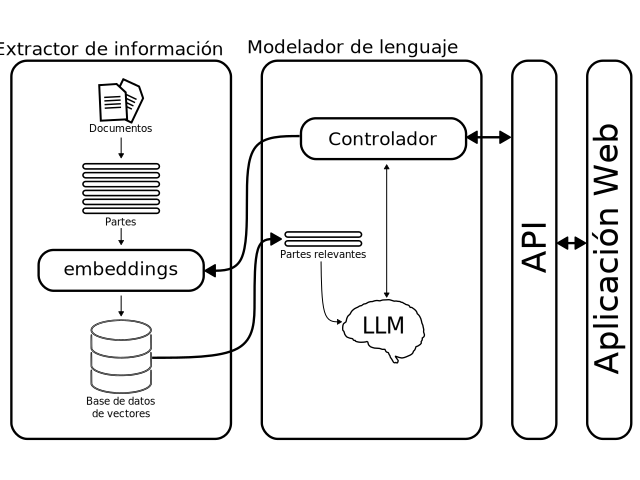
\includegraphics[width = 0.8\textwidth]{\DirFigCtres/esquema_general}
    \caption{Diagrama de componentes que conforman el sistema.}
    \label{fig:esquema_general}
\end{figure}

En las siguientes secciones se explican a detalle cada uno de los componentes.

\section{Extractor de información}

El módulo de extracción de información realiza de una serie de pasos que comienzan con un
archivo en formato PDF y terminan con la creación de una base de datos de
embeddings de cada una de las partes significativas del documento. En la figura
\ref{fig:esquema_extractor} se observa la secuencia de procesamiento del archivo y la
salida de cada una de las etapas.

\begin{figure}[]
    \centering
    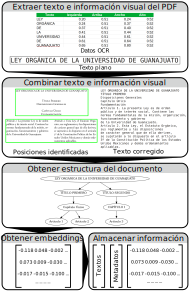
\includegraphics[width = 0.8\textwidth]{\DirFigCtres/esquema_extractor}
    \caption{Diagrama de extracción de información de archivos PDF.}
    \label{fig:esquema_extractor}
\end{figure}

\subsection{Extraer texto e información visual}

El documento PDF no puede procesarse directamente ya que el formato y ubicación
de cada segmento de texto no puede obtenerse de forma confiable,
sin embargo, es necesario contar con esta información para poder extraer la
estructura del documento. Por lo anteior, se extraen dos tipos de datos
del documento: texto plano e información obtenida por OCR (Optical Character
Recognition).

El texto plano se extrae emplendo el modulo PyPDF de Python, el cual lee un archivo
PDF y extrae solamente el texto contenido en él, intentando preservar la secuencia natural
del texto. Sin embargo, este módulo no proporciona información que ayude a
identificar los títulos, secciones y encabezados, además en ocasiones modifica
el orden del texto.

Por otra parte, se utilizan las librerías PDF2Image y PyTesseract para obtener
la información de OCR. La primera permite convertir cada página del archivo PDF
en una imagen de alta resolución, mientras que PyTesseract toma la imagen de la página,
le aplica técnicas de OCR y obtiene información del documento, específicamente,
para cada palabra de la página obtiene: posición, ancho, alto y texto
predicho. Sin embargo, con frecuencia, el texto predicho por PyTesseract es incorrecto,
es por ello que no se puede emplear directamente el texto obtenido.

La librería PyTesseract emplea la herramienta Tesseract, desarrollada por Google,
y es capaz de reconstruir el texto del documento, ya que también detecta las líneas,
párrafos y secciones, sin embargo, con frecuencia comete errores en el ordenamiento
del texto, especialmente en textos de dos columnas, por eso es necesario hacer la
reconstrucción del texto por nuestra cuenta detectando primero renglones,
columnas y secciones como se muestra en la figura \ref{fig:texto_y_ocr}.

\begin{figure}[]
    \centering
    \includegraphics[width = 0.8\textwidth]{\DirFigCtres/esquema_texto_y_ocr}
    \caption{Detalle extracción de texto y características de OCR.}
    \label{fig:texto_y_ocr}
\end{figure}

La tarea de agrupar la página en secciones para posteriormente reconstruir el texto
no es trivial, y es altamente dependiente del tipo de documento del
que se trata, es decir, el proceso descrito en el diagrama de las figuras
\ref{fig:reconstruccion_texto_1} y \ref{fig:reconstruccion_texto_2} funciona para
documentos con estructura similar, donde predomina el texto en una o dos
columnas con títulos centrados.

\begin{figure}[]
    \centering
    \includegraphics[width = 0.8\textwidth]{\DirFigCtres/reconstruccion_texto_ocr_1}
    \caption{Detalle de reconstrucción de información del documento por OCR (Pt. 1).}
    \label{fig:reconstruccion_texto_1}
\end{figure}

\begin{figure}[]
    \centering
    \includegraphics[width = 0.8\textwidth]{\DirFigCtres/reconstruccion_texto_ocr_2}
    \caption{Detalle de reconstrucción de información del documento por OCR (Pt 2).}
    \label{fig:reconstruccion_texto_2}
\end{figure}

Una vez realizada la agrupación de los elementos de la página, es posible reconstruir
el texto respetando el orden normal de lectura. Este texto usualmente contiene
errores de detección que serán corregidos al combinar el texto reconstruido
con OCR con el texto plano extraido con PyPDF.

\subsection{Combinar texto e información visual}

Una vez obtenidos el texto plano y los datos a través de OCR se procede a combinar ambos
elementos, el objetivo es tener la posición de cada palabra asociada con su texto correcto,
de esta forma se podrá distinguir entre diferentes elementos, como títulos, párrafos,
entre otros.

El proceso de combinación requiere las cadenas de texto extraídas por los dos métosos:
la cadena proporcionada por PyPDF y la cadena reconstruida con la información
visual, como se muestra en la figura \ref{fig:texto_y_ocr}. Ambas cadenas se
separan por palabra y se pasan a la librería Difflib, la cual aplica el algoritmo
Ratcliff-Obershelp, también conocido como Coincidencia de patrones Gestalt para
comparar dos cadenas y encontrar sus diferencias.

La razón para dividir el texto en palabras es que el algoritmo compara línea por
línea, pero los saltos de líneas extraidas con PyPDF no siempre conciden con las
extraidas con PyTesseract, por lo que se optó por hacer líneas de una sola palabra.

Si se analizan los patrones de salida de la librería Difflib, es posible
corregir las palabas detectadas con OCR utilizando las palabras extraidas directamente
del texto, los detalles de esta implementación se explican en las figuras
\ref{fig:esquema_combinacion_txt_ocr_1} y \ref{fig:esquema_combinacion_txt_ocr_2}.
En escencia, se considera la palabra obtenida con PyPdf como la correcta,
se compara contra la palabra obtenida con OCR y si es diferente se sobreescribe.

\begin{figure}[]
    \centering
    \includegraphics[width = 0.8\textwidth]{\DirFigCtres/combinacion_texto_ocr_1}
    \caption{Detalle de combinación de teto plano con información de OCR (Pt 1).}
    \label{fig:esquema_combinacion_txt_ocr_1}
\end{figure}

\begin{figure}[]
    \centering
    \includegraphics[width = 0.8\textwidth]{\DirFigCtres/combinacion_texto_ocr_2}
    \caption{Detalle de combinación de teto plano con información de OCR (Pt 2).}
    \label{fig:esquema_combinacion_txt_ocr_2}
\end{figure}

Al terminar el proceso se tiene un arreglo de datos donde se conoce la posición
y dimensiones de cada palabra, así como su texto correcto, además se cuenta con
datos adicionales de linea, columna, alineación o grupo que serán empleadas
para dividir las secciones del documento más adelante.

\subsection{Obtener estructura del documento}

El objetivo de este paso es generar una estructua de datos en la que cada parte
del documento esté referenciada a su sección y subsecciones correspondientes,
por ejemplo, para la Ley Orgánica deseamos conocer en qué título, capítulo y
artículo se encuentra un texto específico.

Para realizar dicha estructura se optó por generar un árbol, donde cada nodo
corresponde a una sección del documento, además, las hojas y los nodos intermedios
almacenan el texto de cada artículo o sección según sea el caso. En la figura
\ref{fig:fragmento_arbol} se muestra un fragmento del árbol correspondiente a
las primeras secciones de la Ley Orgánica.

\begin{figure}[]
    \centering
    \includegraphics[width = 0.8\textwidth]{\DirFigCtres/fragmento_arbol}
    \caption{Fragmento de árbol de documento 'Ley Orgánica de la Universidad de Guanajuato'.}
    \label{fig:fragmento_arbol}
\end{figure}

Para generar el árbol es necesario analizar el documento en varios pasos. Primero,
se detectan las líneas o fragmentos que corresponden a títulos, estas típicamente
se encuentran centrados en la página o en la columna, a los primeros se les
asigna el tipo 1 y a los segundos el tipo 2, el texto restante tendría tipo 0.
Para que el fragmento sea considerado como título deberá haber un espacio
vertical antes o después dependiendo del tipo.

Para encontrar las secciones o subsecciones se consideran los títulos
centrados en la página (tipo 1), a los cuales se les asigna un nivel. Para asignar
el nivel a un título es necesario conocer de antemano la estructura del
documento, específicamente, se debe crear una expresión regular para
identificar cada nivel. Por ejemplo, para la Ley Orgnánica de la Universidad
de Guanajuato la estructura que se tiene es la siguiente:

\begin{enumerate}
    \item Encabezado general: Son títulos abiertos que no tienen palabras o
          estructura específica y se consideran dentro del primer nivel.
          \begin{itemize}
              \item Sin expresión regular
          \end{itemize}
    \item Título: El documento se divide en títulos. Cada título comienza con
          la palabra \textit{Título}.
          \begin{itemize}
              \item \string^(título\textbar[xiv]+\textbackslash.) .*
          \end{itemize}
    \item Capítulo: Los títulos se dividen an capítulos y cada capítulo comienza
          con la palabra \textit{Capítulo}
          \begin{itemize}
              \item \string^capítulo .*
          \end{itemize}
\end{enumerate}

Además, se debe tener en cuenta que hay divisiones del documento
que no se encuentran centrados, sino que están contenidos en el grueso del
texto, como lo son los Artículos. Para identificar estas separaciones en el
contenido, también se crean expresiones regulares que se verifican contra el
inicio de cada línea mientras se va construyendo el árbol.

\begin{enumerate}
    \item Artículo: Los capítulos tienen uno o más artículos.
          \begin{itemize}
              \item  \string^artículo ([0-9]+\textbar[a-zé]+(ro\textbar do\textbar ro\textbar to\textbar mo\textbar vo\textbar no\textbar único)\\
                    (bis\textbar ter\textbar quáter\textbar quinquies)?\textbackslash.
          \end{itemize}
\end{enumerate}

Una vez identificados los títulos y teniendo la forma para encontrar las
divisiones dentro del contenido, se recorre el documento. Recorrer
el documento es el equivalente a recorrer el árbol por profundidad, por lo
que se va creando el árbol de la misma forma, es decir, cuando se encuentra
un título se crea un nuevo nodo en el nivel correspondiente, siempre teniendo
la referencia de cual será su padre, cuando se llega al nivel más bajo se
guarda el contenido de texto en el nodo correspondiente.
El proceso completo se presenta en la figura
\ref{fig:crear_arbol}.

\begin{figure}[]
    \centering
    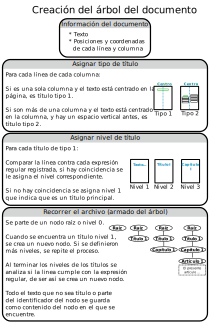
\includegraphics[width = 0.8\textwidth]{\DirFigCtres/crear_arbol}
    \caption{Proceso de creación del árbol de secciones de un documento.}
    \label{fig:crear_arbol}
\end{figure}

\subsection{Obtener embeddings}

Un embedding es una representación de una cadena de texto en un espacio
vectorial de n-dimensiones. Se requiere una red neuronal que tome como entrada
los tokens que conforman la oración y los convierta a un vector numérico,
usualmente esta red es parte de un modelo de lenguaje grande, como puede ser
GPT, Mistral, entre otros, con la diferencia de que se elimina la capa de
predicción del modelo y se usa la salida de la última capa oculta.

Existen librerías que realizan el proceso de tokenizar y convertir a
embeddings utilizando modelos preentrenados, como es el caso de
SentenceTransformers de HuggingFace, el cual dispone de un catálogo ámplio
de modelos de embeddings y con una simple llamada a una función convierte
un conjunto de oraciones en una lista de vectores numéricos.

Al momento se empleó el modelo 'MiniLM-L6-V2', el cual es un modelo pequeño que
devuelve embeddings de 348 valores.

El proceso para convertir la información del documento a embeddings consiste
en recorrer el árbol en profundidad, y en cada nodo hacer lo siguiente:

\begin{enumerate}
    \item Tomar el contenido textual del nodo y separarlo por párrafos.
          Cada párrafo será un registro independiente.
    \item Utilizar SentenceTransformers para calcular los embeddings de cada
          párrafo y guardarlo como un vector de números.
    \item Obtener la ruta del nodo dentro del árbol. Ej: Ley Orgánica $\rightarrow$
          Título Primero $\rightarrow$ Capítulo segundo $\rightarrow$ Artículo 30.
    \item Guardar la ruta y el nombre del nodo como metadatos (información
          adicional que se podría usar para filtrar la información).
\end{enumerate}

Al final por cada párrafo del documento se tendrá la siguiente información:

\begin{itemize}
    \item Metadatos:
          \begin{itemize}
              \item Ruta en el árbol
              \item Nombre del nodo
          \end{itemize}
    \item Embedding como vector de N valores numéricos.
\end{itemize}

\subsection{Almacenar información}

Los embeddings pueden almacenarse de varias formas en el disco, sin embargo,
las dos formas más convenientes son: en formato CSV o en una base de datos
que soporte vectores.

El formato CSV tiene la ventaja de ser portable y facil de leer, lo único que
hay que hacer es convertir los metadatos a formato JSON, así podrán ser
almacenados como texto, mientras que el vector de embeddings se puede
expandir y crear una columna para cada valor. En la figura \ref{fig:ejemplo_csv}
se muestra un ejemplo de la información almacenada como archivo CSV.

\begin{figure}[]
    \centering
    \includegraphics[width = 0.8\textwidth]{\DirFigCtres/ejemplo_csv}
    \caption{Ejemplo de cómo se almacenan metadatos y embeddings en formato csv.}
    \label{fig:ejemplo_csv}
\end{figure}

Sin embargo, este método no es apto para entornos productivos, ya que no tiene
mecanismos nativos para búsqueda en los vectores de datos.

Otra forma de almacenar los embeddings es empleando una base de datos que
soporte vectores. Existen muchas alternativas y cada una ofrece beneficios
particulares, en general todas permiten almacenar los datos de forma
óptima ya que se pueden organizar en tablas, agregar informació adicional y
tienen implementadas funciones de búsqueda por similitud de vectores.
Algunos ejemplos de estas bases de datos vectoriales son: Chroma, Marco,
PostgreSQL, entre otras.

Al momento se han realizado pruebas con ChromaDB, el cual incluye un
mecanismo para calcular los embeddings automáticamente al almacenar los datos
sin tener que hacerlo por separado con SentenceTransformers. En la figura
\ref{fig:ejemplo_chromadb} se muestran los datos almacenados en ChromaDB.

\begin{figure}[]
    \centering
    \includegraphics[width = 0.8\textwidth]{\DirFigCtres/ejemplo_chromadb_1}
    \caption{Ejemplo de cómo se almacenan metadatos en Chroma DB. Los vectores
        se almacenan en un lugar no visible para el usuario.}
    \label{fig:ejemplo_chromadb}
\end{figure}